\documentclass[Orbiter Technical Reference.tex]{subfiles}
\begin{document}

\section{Nonspherical gravitational field perturbations}
\textbf{Martin Schweiger \& Matthew Hume}\\
\textbf{November 18, 2022}


\subsection{Introduction}
Orbiter uses a zonal representation of the gravitational potential generated by a celestial body, using a Legendre polynomial series expansion in the latitude $\theta$. The perturbations in longitude ($\phi$) are assumed to be negligible.
\begin{figure}[H]\centering
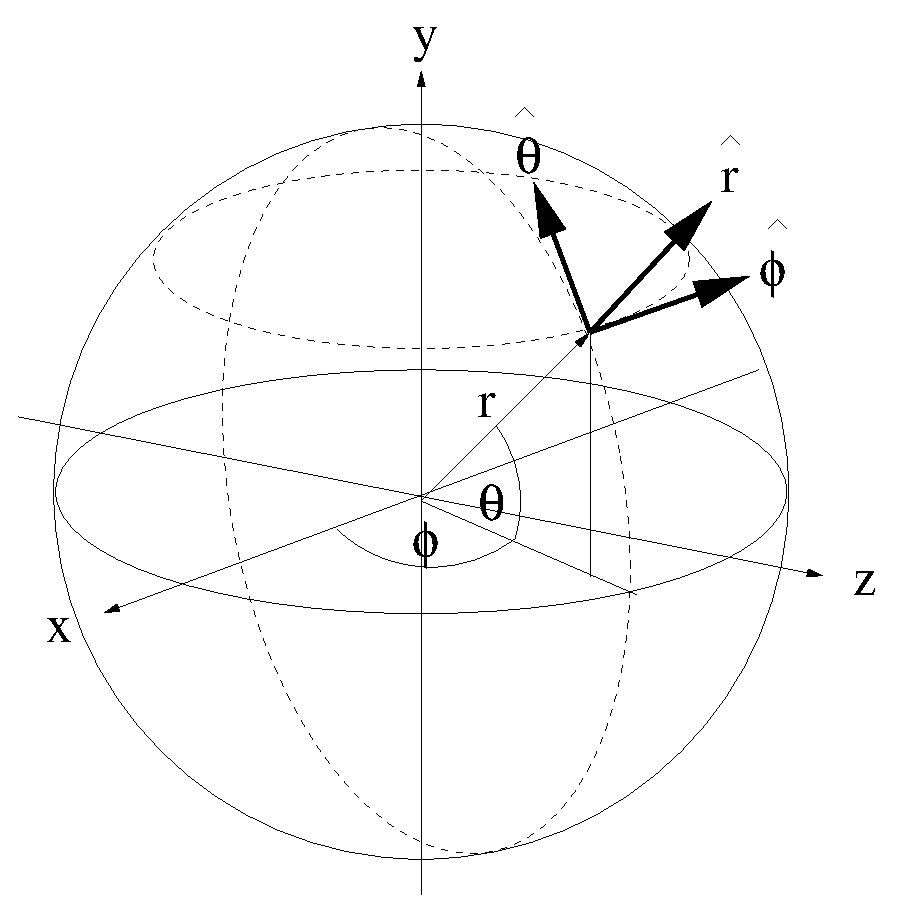
\includegraphics[width=0.45\textwidth]{sphere.eps}
\caption{Planet-relative coordinates and polar unit vectors at a point $(r,\phi,\theta)$.}
\end{figure}
The potential is expressed as
\begin{equation}\label{eq:gpot}
U_G(r,\phi,\theta) = -\frac{GM}{r} \left[ 1 - \sum_{n=2}^\infty J_n \left(\frac{R}{r}\right)^n P_n(\sin \theta) \right]
\end{equation}
where $G$ is the gravitational constant, $M$ and $R$ are the mass and mean radius of the central body, respectively, $r$ is the length of the radius vector, $J_n$ are the coefficients of the series expansion, and $P_n$ are the Legendre polynomials of order $n$.
The first Legendre polynomials are defined as
\begin{equation}
\begin{split}
P_0(x) &= 1\\
P_1(x) &= x\\
P_2(x) &= \frac{1}{2}(3x^2 - 1)\\
P_3(x) &= \frac{1}{2}(5x^3 - 3x)\\
P_4(x) &= \frac{1}{8}(35x^4 - 30x^2 +3)
\end{split}
\end{equation}
The acceleration due to the gravitational field of a test mass at point $\vec{r} = (r,\phi,\theta)$ is then given by the negative gradient of the potential:
\begin{equation}\label{eq:gacc}
\vec{a}_G(r,\phi,\theta) = -\vec{\nabla} U_G(r,\phi,\theta)
\end{equation}
In spherical polar coordinates, the gradient operator is expressed as
\begin{equation}\label{eq:polargrad}
\vec{\nabla} = \hat{r} \frac{\partial}{\partial r} + \frac{1}{r} \hat{\theta}\frac{\partial}{\partial \theta} + \frac{1}{r \cos\theta}\hat{\phi}\frac{\partial}{\partial\phi}
\end{equation}
Substituting equations \ref{eq:gpot} and \ref{eq:polargrad} into \ref{eq:gacc} yields
\begin{equation}
\vec{a}_G(r,\phi,\theta) = \hat{r} a_0^{(r)}(r) - \sum_{n=2}^\infty \left[ \hat{r} a_n^{(r)}(r,\theta) + \hat{\theta} a_n^{(\theta)}(r,\theta) \right]
\end{equation}
with the first terms given by
\begin{equation}
\begin{split}
a_0^{(r)}(r) &= -\frac{GM}{r^2} \\
a_2^{(r)}(r,\theta) &= -\frac{3}{2} \frac{GMR^2 J_2}{r^4}(3\sin^2\theta - 1)\\
a_2^{(\theta)}(r,\theta) &= 3 \frac{GMR^2 J_2}{r^4} \sin\theta \cos\theta \\
a_3^{(r)}(r,\theta) &= -2 \frac{GMR^3 J_3}{r^5}(5 \sin^3\theta - 3\sin\theta)\\
a_3^{(\theta)}(r,\theta) &= \frac{3}{2} \frac{GMR^3 J_3}{r^5} (5 \sin^2\theta \cos\theta - \cos\theta) \\
a_4^{(r)}(r,\theta) &= -\frac{5}{8} \frac{GMR^4 J_4}{r^6}(35 \sin^4\theta - 30\sin^2\theta + 3) \\
a_4^{(\theta)}(r,\theta) &= \frac{5}{2} \frac{GMR^4 J_4}{r^6} (7 \sin^3\theta \cos\theta - 3 \sin\theta \cos\theta)
\end{split}
\end{equation}
The coefficients $J_n$ used by Orbiter are listed in Table~\ref{tab:Jn}.
\begin{table}
\begin{tabular}{lcccc}
        & $J_2$     & $J_3$ & $J_4$ & $J_5$ \\ \hline
Mercury & 60        & -     & -     & -     \\
Venus   & 27        & -     & -     & -     \\ 
Earth   & 1082.6269 & -2.51 & -1.60 & -0.15 \\
Mars    & 1964      & -     & -     & -     \\
Jupiter & 14750     & -     & -     & -     \\
Saturn  & 16450     & -     & -     & -     \\
Uranus  & 12000     & -     & -     & -     \\
Neptune & 4000      & -     & -     & -
\end{tabular}
\caption{Coefficients ($\times 10^6$) for zonal expansion of planetary gravitational potentials.}
\label{tab:Jn}
\end{table}

The field perturbations can lead to a rotation of the orbit trajectory of a satellite. This rotation can be expressed in terms of the movement of the longitude of the ascending node ($\Omega$) and the movement of the argument of periapsis ($\omega$).
If only terms up to $J_2$ are included, approximate values of the movements $\partial\Omega/\partial t$ and $\partial\omega/\partial t$ are given by
\begin{eqnarray}
\frac{\partial\Omega}{\partial t} &=& -\frac{3 n}{2} \left(\frac{R}{a}\right)^2 \frac{\cos i}{(1-e^2)^2} J_2 \label{eq:noderate} \\
\frac{\partial\omega}{\partial t} &=& \frac{3 n}{4} \left(\frac{R}{a}\right)^2 \frac{5 \cos^2 i - 1}{(1-e^2)^2} J_2
\end{eqnarray}
where $n=2\pi/P$ is the mean motion (with orbit period $P$), $a$ is the mean distance, $e$ is the eccentricity, and $i$ is the inclination.

\subsubsection*{Example: calculate the inclination for a sun-synchronous polar orbit}
A sun-synchronous orbits exploits the propagation of the line of nodes to keep the orbital plane synchronised with the relative position of the sun. A satellite can for example be placed in a sun-synchronous orbit so that it continuously flys over the planet's terminator line.
From~\ref{eq:noderate} we have
\begin{equation}
\cos i = -\frac{2}{3 n} \left(\frac{a}{R} \right)^2 \frac{(1-e^2)^2}{J_2} \frac{\partial\Omega}{\partial t}
\end{equation}
A sun-synchronous orbit requires the line of nodes to move at a rate of $2\pi$ per year. For Earth, this is equivalent to $\partial\Omega/\partial t = 1.99\cdot 10^{-7}$\,rad/s (about $0.99$ deg. per day). Assume a circular orbit ($e=0$) at an altitude of 300\,km
%($a = 6 678 137$\,m, with $R_E = 6 378 137$\,m).
($a = 6 671 010$\,m, with $R_E = 6 371 010$\,m).
With $P = 2\pi\sqrt{a^3/\mu_E}$ we get $n = \sqrt{\mu_E/a^3} = 0.0012$\,rad/s. This leads to
\begin{equation}
\cos i_\text{sync} = -\frac{2}{0.0035} \left(\frac{6 678 137}{6 378 137}\right)^2 \frac{1.99\cdot 10^{-7}}{0.001082630} = -0.116,
\end{equation}
or $i_\text{sync} = 96.7$\,deg.
%
%	Section added by M. Hume
%
\subsection{Extension to Tesseral Harmonics}
In some cases neglecting the variation in perturbation with longitude is insufficient. Long-term evolution of orbital parameters and the degree to which vessel position and velocity retain a high degree of congruence with real-world observations and with other state vector propagation software, require gravity model that depends on both latitude and longitude.
This accomplished by replacing the zonal terms previously discussed with tesseral terms. A tesseral gravity model includes non-spherical perturbation that vary continuously with both latitude and longitude. Where zonal terms can be represented as an ordered list of terms, tesseral terms are represented in the following form, $C(n,m)$ and $S(n,m)$ where , $0 \leq n \leq n_\text{max}$ and $0 \leq m \leq n$.
A conventional representation of a harmonic gravitational potential is shown below, Pines\cite{pines73}(3), note the similarities to (1).
\begin{equation}
U_G(r,\phi,\theta) = \frac{\mu}{r}\left\{1+\sum_{n=1}^{\infty}\left ( \frac{a}{r} \right )^n \sum_{m=1}^{n}P_{n,m}(sin (\theta))(C_{n,m}cos(m\phi)+S_{n,m}cos(m\phi)) \right\}
\end{equation}
Pines\cite{pines73} transforms this representation, such that the singularities present at the poles and the non-uniformities in numerical precision that would result in their vicinity in a computational representation are eliminated. Pines\cite{pines73} uniform representation of the gravitational potential is:
\begin{equation}
U_G(s, t, u) = \frac{\mu}{r}\left\{1+\sum_{n=1}^{\infty}\left ( \frac{a}{r} \right )^n \sum_{m=1}^{n}A_{n,m}(u)(C_{n,m}r_m(s,t)+S_{n,m}i_m(s,t)) \right\}
\end{equation}
where s, t, and u are the x, y, and z\footnote{Note: Orbiter uses a left-handed coordinate system, wherein the y and z axes are swaped with respect conventional systems like IAU.}, components of position normalized by the magnitude of the position vector, $r_m(s,t)$ and $i_m(s,t)$  are the real and imaginary components respectively of $(s+it)^m$, and $A_{n,m}(u)$ are the \emph{m}th derivative of the associated Legendre polynomial $P_{n,m}(u)$.
Similar to the zonal representation, the acceleration vector acting upon the spacecraft is found by computing the gradient of the potential. The algorithm used to compute acceleration is discussed and described in detail by Eckman et al.\cite{Eckman08}, referencing the implementation developed by DeMars et al.\cite{DeMars08}

\subsubsection{Notes on Usage}
Gravity models must follow certain conventions in order to be used. The format used by this implementation is the SHADR format, or Spherical Harmonic ASCII Data Record of PSI\cite{shadr}. Only ASCII models where degree = order are supported.
The first line of a model file is the header and consists of properties for the entire model. All subsequent lines contain data for harmonics coefficients. Details of the header line format can be found in Table~\ref{tab:headlinefmat}
\begin{table}[h]
\begin{tabular}{llcc}
Column	&Parameter                        				&Units      			& Notes     \\\hline
1		&Reference Radius                 				&km         			&           \\
2		&Standard Gravitational Parameter 			&km$^3$/sec$^2$ 	&           \\
3		&Uncertainty in Standard Gravitational Parameter	&none           		& Not used. \\
4		&Degree of Field						&none           		&		\\
5		&Order of Field						&none				&		\\
6		&Normalization Status					&none				&Must be 1	\\
7		&Reference Latitude					&Degrees			&Must be 0	\\
8		&Reference Longitude					&Degrees			&Must be 0	
\end{tabular}
\caption{Gravity Model Header Line Format}
\label{tab:headlinefmat}
\end{table}


An example of a header line from the LP165 model is shown below.
\begin{tiny}
\begin{verbatim}
  .17380000000000E+04,  .49028010560000E+04,  .21700000000000E-03,  165,  165,    1,  .00000000000000E+00,  .00000000000000E+00   
\end{verbatim}
\end{tiny}

Subsequent lines contain the $C(n,m)$ and $S(n,m)$ coefficients. Details on the coefficient lines can be found in Table~\ref{tab:coefflinefmat}

\begin{table}[h]
\begin{tabular}{llcc}
Column	&Parameter                        				&Units      			& Notes     \\\hline
1		&n                							&none        			&           \\
2		&m 								&none 			&           \\
3		&$C(n,m)$							&none           		&  \\
4		&$S(n,m)$ 							&none           		&		\\
5		&Uncertainty in $C(n,m)$	 				&none				&Not used		\\
6		&Uncertainty in $S(n,m)$					&none				&Not used	
\end{tabular}
\caption{Gravity Model Header Line Format}
\label{tab:coefflinefmat}
\end{table}



An example of lines defining the harmonic coefficients are shown below.
\begin{tiny}
\begin{verbatim}
    1,    0,  .0000000000000000E+00,  .0000000000000000E+00,  .0000000000000000E+00,  .0000000000000000E+00             
    1,    1,  .0000000000000000E+00,  .0000000000000000E+00,  .0000000000000000E+00,  .0000000000000000E+00             
    2,    0, -.9089018075060000E-04,  .0000000000000000E+00,  .5462525382390000E-08,  .0000000000000000E+00             
    2,    1, -.2722032361590000E-08, -.7575182920830000E-09,  .4505315582830000E-08,  .3485921417110000E-08             
    2,    2,  .3463549937220000E-04,  .1672949053830000E-07,  .3684587359180000E-08,  .3042220665000000E-08             
    3,    0, -.3203591400300000E-05,  .0000000000000000E+00,  .6482991943890000E-08,  .0000000000000000E+00             
    3,    1,  .2632744012180000E-04,  .5464363089820000E-05,  .7496882504270000E-08,  .4465401948060000E-08             
    3,    2,  .1418817932940000E-04,  .4892036500480000E-05,  .6742524852930000E-08,  .6037402771920000E-08             
    3,    3,  .1228605894470000E-04, -.1785448081640000E-05,  .4519014367070000E-08,  .4568425931770000E-08             
\end{verbatim}
\end{tiny}
New gravity models must be added to the folder \emph{./GravityModels}, the corresponding body configuration file must be edited to include the following lines:
\begin{tiny}
\begin{verbatim}
; === Gravity Models ===
; ref: see Doc/Orbiter Technical Reference.pdf for details on implementation and usage
GravModelPath = jgl165p1.sha       ; the name of the gravity model file to load, located in /GravityModels
GravCoeffCutoff = 10               ; the maximum number of terms to load.
\end{verbatim}
\end{tiny}
\paragraph{Limitations}
All gravity models must start with the C(1,0) and S(1,0) coefficients. In the case that they have been omitted by the original creator of the model, they must be padded by zeros as shown in the first two lines of the example above. Additionally: only normalized coefficients are supported, only models that have a reference latitude and longitude corresponding to Orbiter's positive X axis are supported (latitude = 0°, longitude = 0°).

\paragraph{Included Models}
By default Orbiter comes with four gravity models, one each for: Mercury, Venus, Earth, Luna, Mars, and Vesta. The default cut-off degree/order is 10 to minimize the impact on simulation performance, however this can be increased at the users discretion. A summary of the models included with this release and their respective default settings is shown in Table~\ref{tab:models}
\begin{table}[h]
\begin{tabular}{llcc}
Body    	& Model                 					& Maximum Degree/Order 		& Default Degree/Order \\\hline
Mercury 	& \emph{jgmess\_160a\_sha.tab} 		& 160                  			& 10                   \\
Venus   	& \emph{mod\_shgj120p.a01}     		& 120                  			& 10                   \\
Earth   	& \emph{egm96\_to360.tab}     			& 360                 			& 10                   \\
Luna    	& \emph{jgl165p1.sha}				& 165                  			& 10                   \\
Mars    	& \emph{jgmro\_120f\_sha.tab}  		& 120                  			& 10		     \\
Vesta    	& \emph{JGDWN\_VES20H\_SHA.TAB}		& 20                  			& 10
\end{tabular}
\caption{Gravity models included with Orbiter}
\label{tab:models}
\end{table}

\subsubsection{Testing and Results}
A test was devised using NASA JPL's GMAT software package to produce control. A simulation was set up consisting of a spacecraft in a 45\textdegree inclination orbit around Earth's Moon, approximately 75x62km. The orbit was propagated for $10^5$ seconds while logging state vector. For control, the GMAT propagator was set to RungeKutta89 with an accuracy of $1\times10^{-13}$ and the RSSStep error control method. The gravity model \emph{jgl165p1.sha} was used with the coefficient cut-off set to the maximum value of 165. In Orbiter, the propagator was set to RK8. Both simulations used fixed 5 second time-steps. 

Figure~\ref{fig:alt} show GMAT altitude above the mean Lunar surface, overlaid on the results from the Orbiter model as a comparison. Trends in apoapsis and periapsis height, and eccentricity are highly congruent between the two models. To quantify the relative error in the Orbiter implementation, the difference in position in the rotating lunar reference frame was computed and is plotted in Figure~\ref{fig:error}. A second test was carried out, recording position in both GMAT and Orbiter with point-mass gravity only. The difference in the error between these two test runs is plotted in Figure~\ref{fig:errordiff}, and was observed to be several orders of magnitude less than the absolute position error with or without complex gravity.

Further work is needed to quantify the absolute position error between Orbiter and GMAT. The source of this error is believed to be differences in propagators and error control between GMAT and Orbiter. Changing propagator settings had the largest effect on the magnitude of the error plotted in Figure~\ref{fig:error}. Two models for Lunar position and rotation were tested, both Orbiter's default ELP82 and JPL's DE440, however neither had significant impact on reducing the error. Given the relatively small difference in error between the test case with point-mass gravity and with complex gravity, there is a high degree of confidence in the acceleration values this model produces.

Further details on ephemeris models can be found at \url{https://www.orbiter-forum.com/threads/improved-tesseral-gravity-model.40266/post-603043}

\begin{figure}[H]
\centering
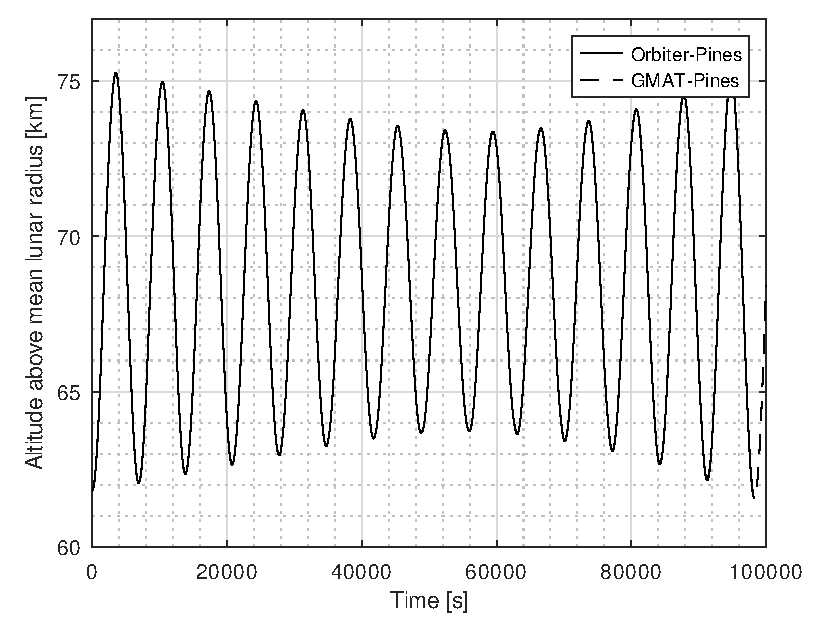
\includegraphics[width=1.0\textwidth]{altitude.eps}
\caption{Comparison of Orbiter-Pines and GMAT Altitude above Mean Lunar Radius}
\label{fig:alt}
\end{figure}

\begin{figure}[H]
\centering
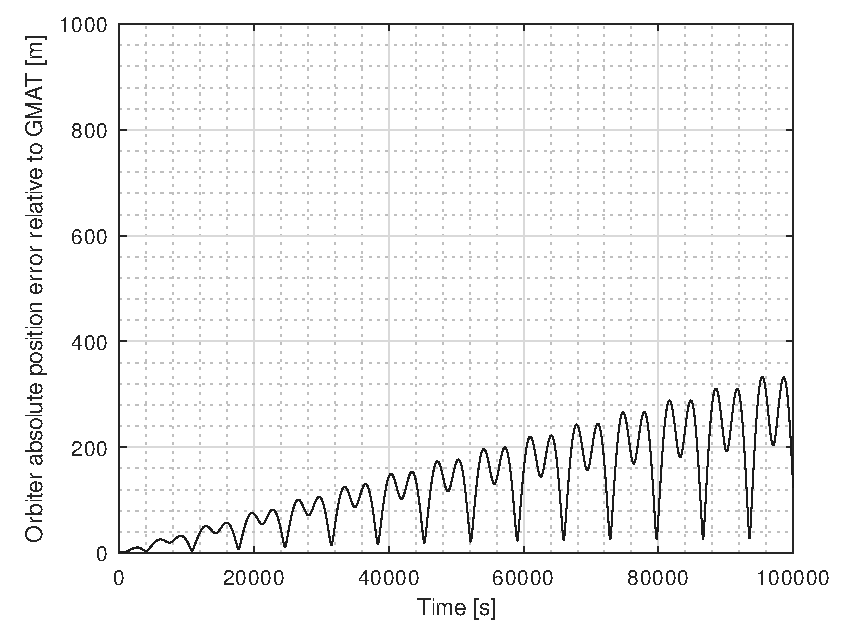
\includegraphics[width=1.0\textwidth]{position_error}
\caption{Comparison of Position Relative to Rotating Lunar ReferenceFrame}
\label{fig:error}
\end{figure}

\begin{figure}[H]
\centering
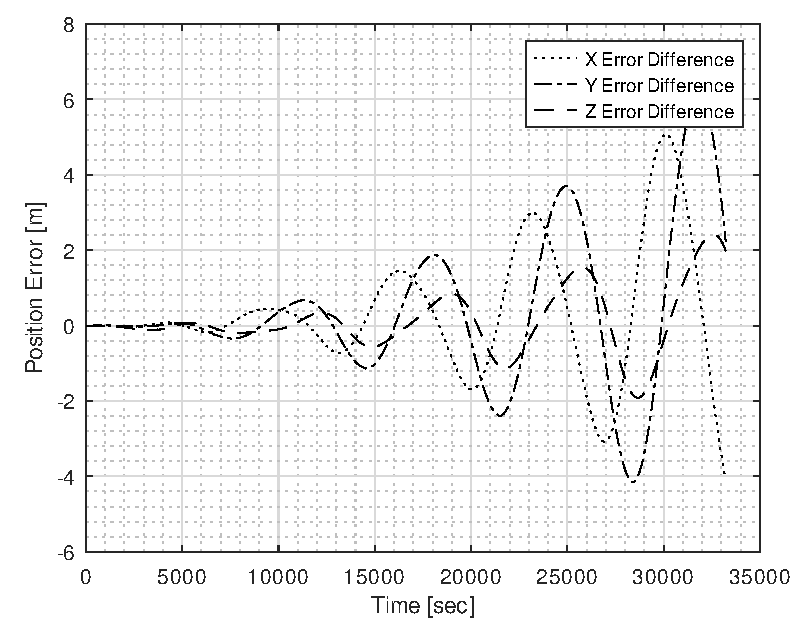
\includegraphics[width=1.0\textwidth]{errordiff.eps}
\caption{Difference Between Position Error with and without Complex Gravity}
\label{fig:errordiff}
\end{figure}

\end{document}
